Deep neural networks typically have a large upfront cost associated with computational power and training dataset size. Even with modern training optimization algorithms such as Stochastic Gradient Descent~\cite{SGD}, training cost poses the biggest obstacle to achieving higher test accuracy. The advent GPU-based parallel processing has contributed the most to surpassing this obstacle, allowing previously impractical networks to become possible. For instance, training state-of-the-art NN's like BERT~\cite{bert} and ResNet-50~\cite{resnet} were able to be done in 3 days and 29 hours, respectively, as opposed to the original training time of several weeks. This feat was not possible even with the largest scale server processors before the beginning of this decade. 

Recent research in lowering training cost has been focused on optimizing the actual mathematical calculations during the process. Methods to make minor improvements include choosing optimal hyperparameters like the learning rate, automated perceptron pruning/dropout[], and by applying some form of gradient normalization. More complicated adaptive approaches attempt to better understand the direction of negative gradient to achieve more effective steps, typically using moving averages of the first and second moments. Popular optimizers like Adam and AdamW incorporate this adaptive approach and have shown substantial improvements over its predecessors[]. More advanced algorithms such as LAMB~\cite{You2020Large}, LARS~\cite{qian2020impact, ginsburg2018large}, or NVLAMB~\cite{nvidia_nvlamb}  take this mentality several steps further and apply layer-wise adaptive gradient pre/normalization. This paper shall investigate, compare, and implement these innovative optimization techniques in relation to deep NN's in the NLP and Image Processing domain. 

\begin{figure}[!t]
    \centering
    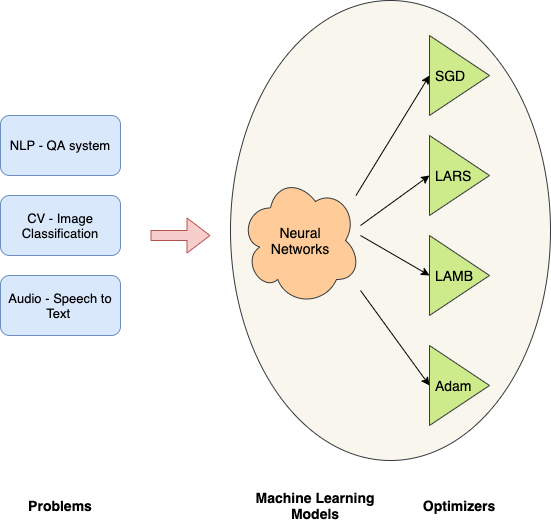
\includegraphics[width=\linewidth, height=7.5cm]{img/dl_optimizers.png}
    \caption{Type of problems in this study across four state-of-the-art optimizers}
    \label{fig:study}
    \vspace{-10pt}
\end{figure}

Image classification is a process of labeling and categorizing pictures. For most image classification tasks, convolutional neural networks are the most effective at achieving high accuracy with a moderate number of perceptron connections. However, with recurrent convolutional and pooling layers, these networks can become very deep (large number of parameters) relatively quickly[]. Many issues arise with standard back-propagation techniques of these deep CNN's, putting a large burden on the effectiveness of the optimizer chosen to train the model. Even after thousands of iterations and epochs, some optimizers still fail converge to optimal weights[] with used on models with high numbers of layers. We expect that the layer-wise approach taken by the LAMB or LARS optimizers will thus improve training time of these types deep networks significantly, as they should be able to better incorporate information from the individual layer gradients. This decrease in training time should be seen as a faster decrease in the loss function value while still maintaining relatively similar accuracy on the test/validation set.

Another common application of machine learning is the use of NN's for speech-to-text transcription. This involves transforming raw audio signals into human-readable text. Consumer products such as the Amazon Alexa, Siri from Apple, the Google Assistant all utilize the most cutting-edge speech-to-text models. These models are usually multimodal but are based on some form of a Hidden Markov Model (HMM)[]. Preproccessing of the input data is usually done by dividing the speech signal into segmented chunks and applying signal processing transforms (FFT)[]. This makes speech recognition algorithms very computationally expensive and incorporate extremely large numbers of trainable parameters. We expect that optimizer's like LAMB/LARS could help reduce this computational cost of training when used on modern speech-to-text architecture such as the LAS model[].

The final type of machine learning model tested in this paper will be a question answering (QA) system, which belongs to the category of information retrieval. These systems consist of three parts: question classification, information retrieval, and answer extraction. Since these models  must be able to respond with a large vocabulary and are very dynamic in nature, they usually suffer from extremely large training times. The overall architecture of the model we will test will include a LSTM network with attention, which is the standard model used in production. We believe that the application of layer-wise adaptive scaling and prenormalization will improve the initial loss decrease and allow for larger batch-size/distributed training.\\






% \begin{table}[!t]
% \vspace{-15pt}
% \scriptsize
% \vspace{7pt}
% \caption{Plan of project work.}\label{tbl:planofwork}
% \vspace{-15pt}
% \begin{center}
% \begin{tabular}{ l|c|l}
%   \multicolumn{1}{c|}{Standard} &
%  \multicolumn{1}{c|}{Date} &
%  \multicolumn{1}{c}{Responsibilities}\\
%  %& & \\
% \hline
% & & We will research necessary papers and  \\
%  Literature Review & 9/07 - 9/25 &  contribute information to address how the  \\
%  & &  problem relates to the group's interests. \\\hline
% & & Each of us will propose appropriate \\
% Experiment Setup & 	09/25 - 10/02 & application, setting, and dataset for this\\
% & &  project's direction.\\\hline
% & & We will delegate coding parts based off of \\
% Implementation & 10/02 - 10/16  & each individual's strength (e.g. each optimizer \\
% & & per individual group member) \\\hline
% & & We will share the exploration of applicable \\
% Mathematical and & 10/16 - 10/30 &  theories (e.g. LARS \& LAMB) while \\ 
% Result Analysis & &	  evaluate the results deeply in regards to  \\
% & & the problem's context\\\hline
% & & Each of us will help report background \\
% Documentation & 10/30 - 11/13 &  theories, outcomes, discussion, and possible\\
% & &  future directions. \\


% \end{tabular}
% \end{center}
% \vspace{-15pt}
% \end{table}